In this thesis, a first demonstrator of a new \gls{daq} system based on the photonic time-stretch method was developed.
The system consists of a high bandwidth front-end sampling card, mounted on a new generation of \gls{rfsoc} for readout of the acquired samples. 
The sampling card was designed to fully exploit all the features of the \gls{rfsoc}. 
\begin{itemize}
	\item Integrated high-speed \glspl{adc} with 14-bit resolution and a sample rate up to \SI{2.5}{\giga \sample \per \second}. With the sixteen available converters and using a time-interleaving method, the system is capable of a sample rate of \SI{40}{\giga \sample \per \second}, allowing a continuous sampling with high temporal resolution.
	\item On-chip \gls{fpga} provides high-speed control and the flexibility adjust the firmware to user needs.
	\item On-chip memory to intermediately store acquired data.
	\item The \gls{soc} high-speed connections (e.g. 100G-Ethernet) in order to guarantee the high-speed throughput of the data (range of TeraBits!)
	\item Use of the provided framework in order to quickly characterize system performance
\end{itemize}

The system can be used to assist research in important scientific topics, e.g. improving quality of beam diagnostics or the research of laser dynamic.
Potential industrialization of the \gls{daq} is also foreseen. 


%There is a disturbing lack of benches in \sout{Ramset Park} Campus North. I want to sit more!
%
%\begin{figure}[tbh]
%	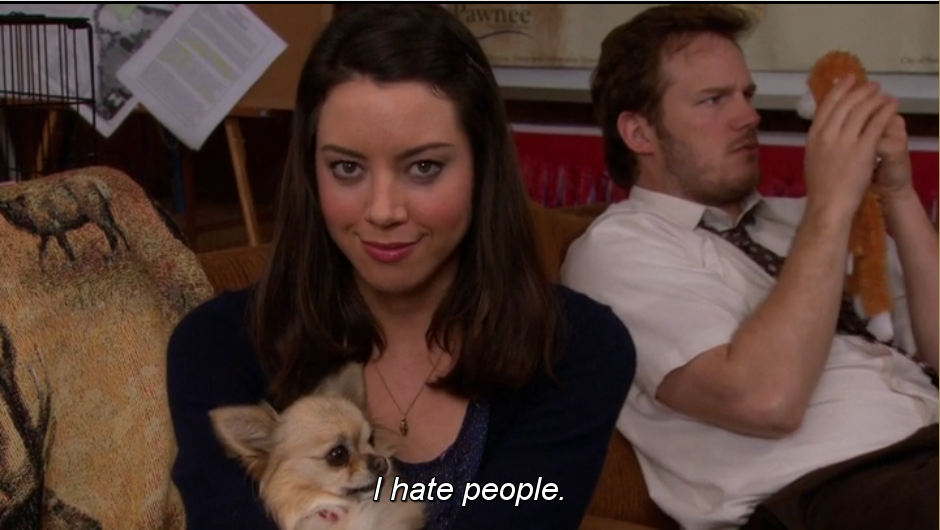
\includegraphics[width=\textwidth]{chap/06-conclusion/img/april}
%\end{figure}
%
%\newpage
%\section{Expectation vs. Reality}
%At least I wrote more than 273 words.
%\begin{figure}[tbh]
%     \centering
%     \begin{subfigure}{0.7\textwidth}
%         \centering
%         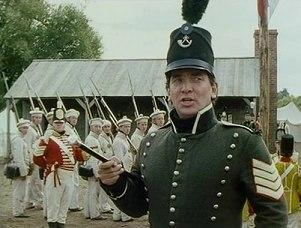
\includegraphics[width=\textwidth]{chap/06-conclusion/img/harper}
%         \caption{How you think you will feel like at the end of your master studies.}
%         \label{fig:expectation}
%     \end{subfigure}
%     
%     \begin{subfigure}{0.7\textwidth}
%         \centering
%         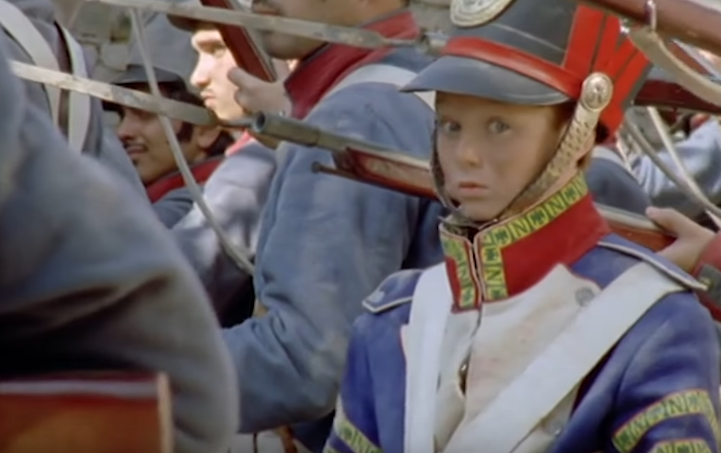
\includegraphics[width=\textwidth]{chap/06-conclusion/img/bubi}
%         \caption{How you actually feel like.}
%         \label{fig:reality}
%     \end{subfigure}
%     \caption{Expectation vs. Reality}
%\end{figure}
%
%
%
%\section{The board}
%\begin{figure}[H]
%	\centering
%	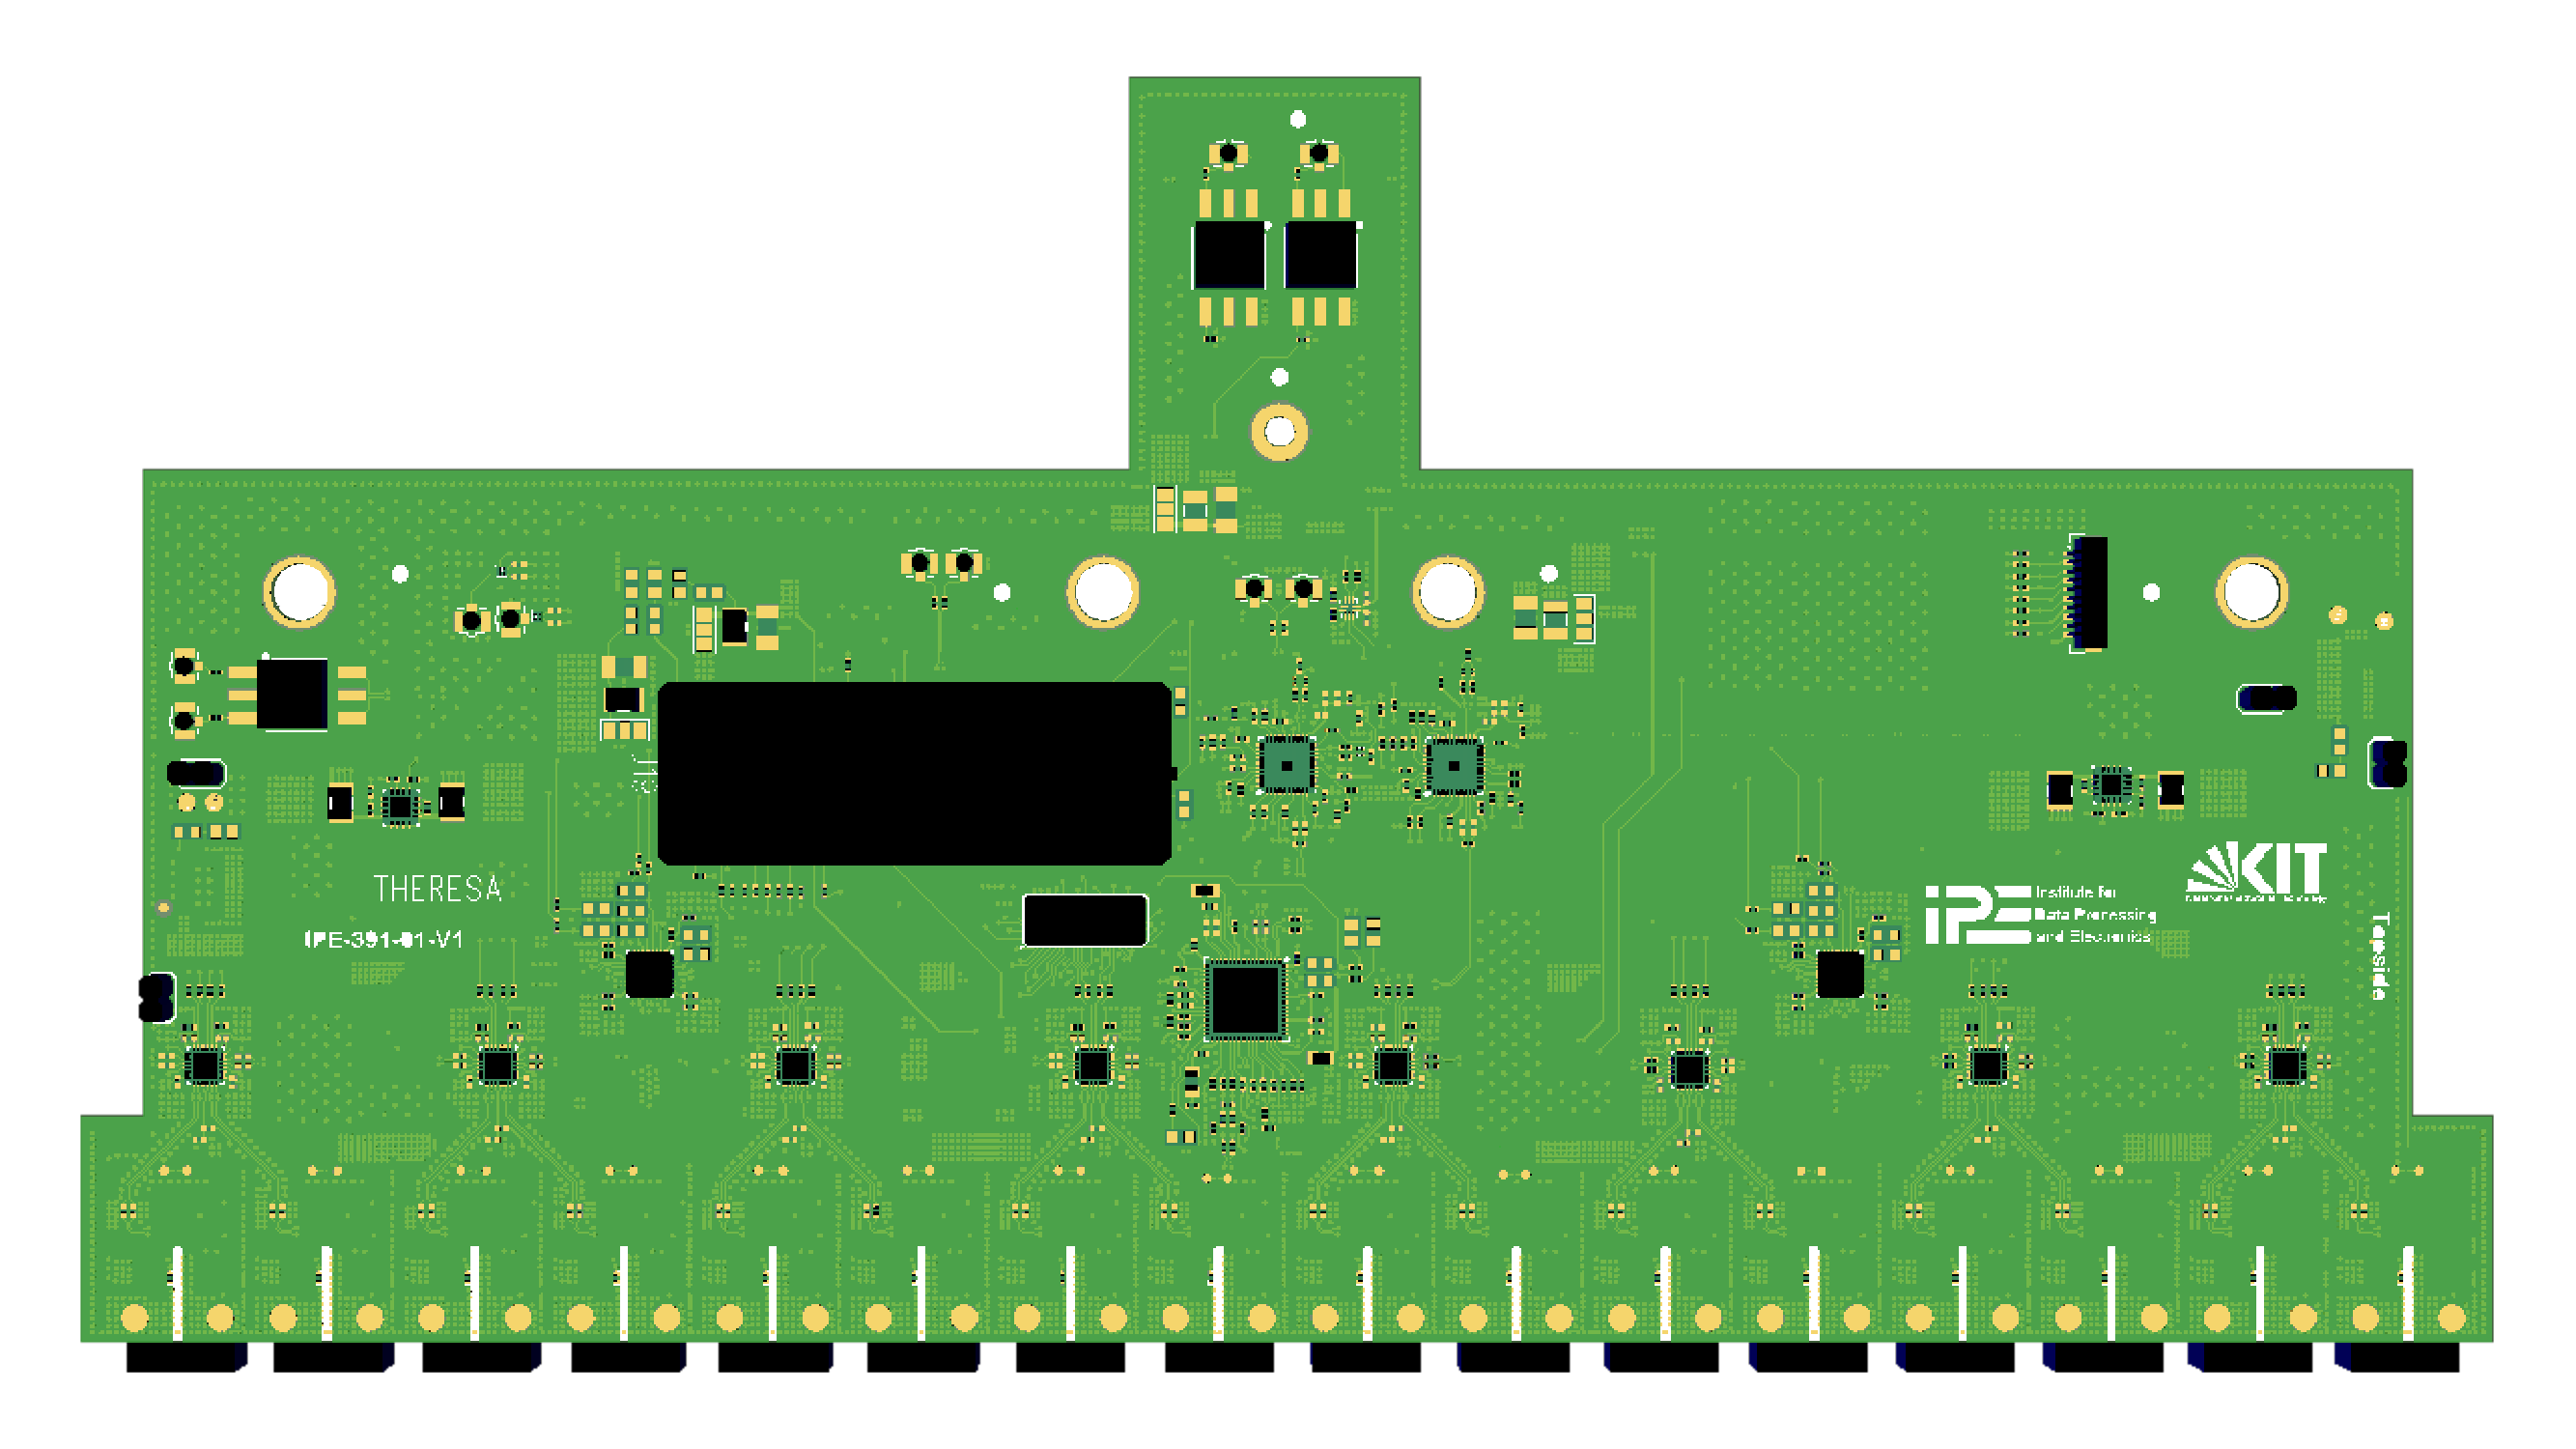
\includegraphics[width = \textwidth]{chap/06-conclusion/img/board}
%	\caption{THERESA}
%	\label{fig:board}
%\end{figure}
